
%%%%%%%%%%%%%%%%%%%%%%%%%%%%%%%%%%%%%%%%%%
%%                                      %%
%%          Resultados Obtidos          %%
%%                                      %%
%%%%%%%%%%%%%%%%%%%%%%%%%%%%%%%%%%%%%%%%%%

% Neste capítulo são expostos os resultados de sua pesquisa. 
% No caso do TCC I, resultados esperados ou parciais, para TCC II, resultados "finais".

\chapter{Resultados}
    \label{cha:resultados}
    Neste capítulo serão discutidos os resultados obtidos após a aplicação da proposta discutida no Capítulo~\ref{cha:desenvolvimento-da-pesquisa}.
    A abordagem deste capítulo possui dois momentos, o primeiro momento, descrito na Seção~\ref{sec:performance-analysis}, onde são apresentados os resultados obtidos por cada classificador individualmente e também são realizadas análises no parâmetro $cr$ por classificador, por cada variação do algoritmo \ac{flexcon}. Por fim, no segundo momento, Seção~\ref{sec:statistical-analysis}, foi conduzida uma análise estatística dos resultados obtidos.
    
    % Pegar dados do Planilhas do Google Drive e transforma-los em gráficos de linhas onde o eixo X representa a porcentagem de inicialmente rotulados, o Y a porcentagem da acurácia do algoritmo e a linha representa a porcentagem de variação do limiar
    
    % Como resultados parciais deste trabalho destacam\hyp{se} a aplicação de três taxas de variações (3\%, 5\% e 7\%) que manipulam o limiar da iteração seguinte. O algoritmo \textit{FlexCon\hyp{C1} (v)} foi aplicado a um conjunto de três bases de dados (\textit{Mammographic Mass}, \textit{Mfeat\hyp{karhunen}} e \textit{Mushroom}). A Tabela~\ref{tab:partial-results} apresenta as acurácias obtidas para cada uma das bases de dados utilizando o algoritmo \textit{FlexCon\hyp{C1} (v)} aliado ao classificador Naive Bayes.
    
    % \begin{table}[h]
    %     \centering
    %     \caption{Acurácia do \textit{FlexCon\hyp{C1} (v)} utilizando o classificador Naive Bayes.}
    %     \label{tab:partial-results}
    %     \resizebox{\textwidth}{!}{%
    %         \begin{tabular}{|c|c|c|c|c|c|c|}
    %             \toprule
    %             \multirow{2}{*}{\textbf{Base de Dados}}     & \multirow{2}{*}{\textbf{Taxa de Variação}} & \multicolumn{5}{c|}{\textbf{Inicialmente Rotulados}} \\ \cmidrule(l){3-7} 
    %                                               &                                   & \textbf{5\%}     & \textbf{10\%}   & \textbf{15\%}   & \textbf{20\%}   & \textbf{25\%}   \\ \midrule
    %             \multirow{3}{*}{Mammographic Mass} & 3\%                               & 75.83\%   & 75.42\%  & 77.08\%  & 75.83\%  & 77.92\%  \\ \cmidrule(l){2-7} 
    %                                               & 5\%                               & 75.83\%   & 75.42\%  & 77.08\%  & \textbf{76.25\%}  & 77.92\%  \\ \cmidrule(l){2-7} 
    %                                               & 7\%                               & 75.83\%   & 75.42\%  & 77.08\%  & 75.83\%  & 77.92\%  \\ \midrule
    %             \multirow{3}{*}{Mfeat\hyp{karhunen}}    & 3\%                               & 84.60\%   & 88.00\%  & 90.20\%  & \textbf{90.60\%}  & 89.40\%  \\ \cmidrule(l){2-7} 
    %                                               & 5\%                               & \textbf{85.40\%}   & \textbf{88.60\%}  & \textbf{91.20\%}  & \textbf{90.60\%}  & \textbf{90.00\%}  \\ \cmidrule(l){2-7} 
    %                                               & 7\%                               & 84.60\%   & 88.00\%  & 90.20\%  & 90.40\%  & 89.40\%  \\ \midrule
    %              \multirow{3}{*}{Mushroom}          & 3\%                               & 89.66\%   & 90.89\%  & 91.68\%  & 90.65\%  & \textbf{93.11\%}  \\ \cmidrule(l){2-7} 
    %                                               & 5\%                               & \textbf{90.74\%}   & \textbf{92.12\%}  & \textbf{92.27\%}  & \textbf{91.97\%}  & 92.61\%  \\ \cmidrule(l){2-7} 
    %                                               & 7\%                               & 89.66\%   & 90.50\%  & 91.19\%  & 91.04\%  & 91.29\%  \\ \bottomrule
    %         \end{tabular}
    %     }
    %     \source{O Próprio Autor (\imprimirdata)}
    % \end{table}
    
    % As Figuras~\ref{fig:base-mammographic}, \ref{fig:base-mfeat-karhunen} e \ref{fig:base-mushroom} apresentam gráficos sintetizando as informações contidas na Tabela~\ref{tab:partial-results} para as bases de dados \textit{Mammographic Mass}, \textit{Mfeat\hyp{karhunen}} e \textit{Mushroom} respectivamente. Nestes gráficos estão representados os percentuais de exemplos inicialmente rotulados pelas acurácias obtidas alterando a taxa de variação do limiar.
    
    % \begin{figure}[h]
    %     \centering
    %     \caption{Percentuais de Exemplos Inicialmente Rotulados x Acurácia Obtida na Base \textit{Mammographic Mass}.}
    %     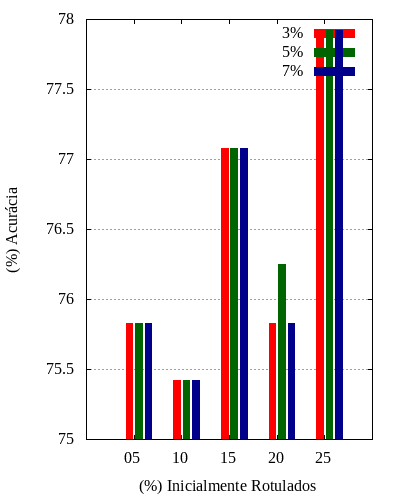
\includegraphics[scale=0.5]{figuras/Mammographic.png}
    %     \label{fig:base-mammographic}
    %     \source{O Próprio Autor (\imprimirdata)}
    % \end{figure}
    
    % \begin{figure}[h]
    %     \centering
    %     \caption{Percentuais de Exemplos Inicialmente Rotulados x Acurácia Obtida na Base \textit{Mfeat\hyp{karhunen}}.}
    %     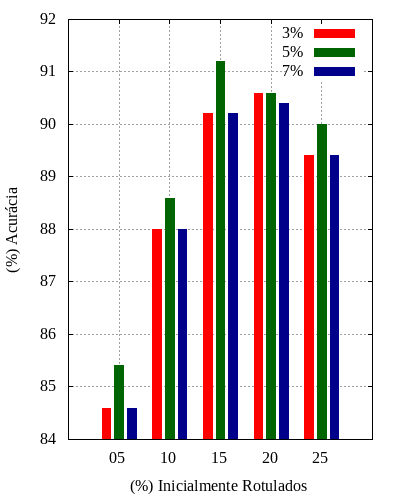
\includegraphics[scale=0.5]{figuras/Mfeat-karhunen.png}
    %     \label{fig:base-mfeat-karhunen}
    %     \source{O Próprio Autor (\imprimirdata)}
    % \end{figure}
    
    % \begin{figure}[h]
    %     \centering
    %     \caption{Percentuais de Exemplos Inicialmente Rotulados x Acurácia Obtida na Base \textit{Mushroom}.}
    %     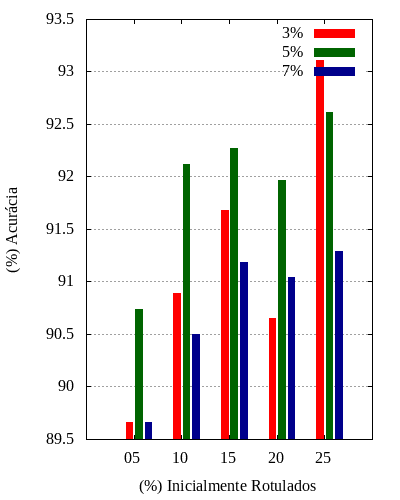
\includegraphics[scale=0.5]{figuras/Mushroom.png}
    %     \label{fig:base-mushroom}
    %     \source{O Próprio Autor (\imprimirdata)}
    % \end{figure}
    
    % As Tabelas~\ref{tab:naive-acc}-\ref{tab:knn-acc} apresentam em cada uma das células as acurácias médias obtidas pelos classificadores, além de apresentar também o desvio padrão obtido por cada classificador (Na\"ive Bayes, \textit{rpartXse}, \ac{ripper} e \ac{knn}), respectivamente. Em cada uma das referidas tabelas, está sendo analisado a variação do parâmetro $cr$ em diferentes algoritmos e diferentes percentuais de exemplos rotulados.
    \section{Analise de Performance}
        \label{sec:performance-analysis}
        
        As Tabelas~\ref{tab:naive-acc}-\ref{tab:knn-acc} apresentam o desempenho obtido pelo algoritmo \ac{flexcon} em cada uma das suas variações. Nestas tabelas, as colunas são as variações aplicadas ao parâmetro $cr$ das células as acurácias médias obtidas pelos classificadores, além de apresentar também o desvio padrão obtido por cada classificador (Na\"ive Bayes, \textit{rpartXse}, \ac{ripper} e \ac{knn}), respectivamente. Em cada uma das referidas tabelas, está sendo analisado a variação do parâmetro $cr$ em diferentes algoritmos e diferentes percentuais de exemplos rotulados.
        
        A Tabela~\ref{tab:naive-acc} apresenta os resultados obtidos após a aplicação do classificador Na\"ive Bayes. Os melhores resultados encontram\hyp{se} entre 2\% a 4\%. Realizando uma análise por algoritmo, observa\hyp{se} que quando pré\hyp{fixa} o valor do parâmetro $cr$ em 3\% obtém\hyp{se} resultados superiores em 3 dos 5 casos, para os três algoritmos. De maneira geral quando o valor do parâmetro $cr$ é pré\hyp{fixado} em 3\% os resultados são superiores em 9 dos 15 casos, representando 60\% de superioridade.
    
    \begin{table}[h]
        \centering
        \caption{Resultado da acurácia com o classificador Na\"ive Bayes}
        \resizebox{\textwidth}{!} & \textbf{3\%} & \textbf{4\%} & \textbf{5\%} & \textbf{6\%} & \textbf{7\%} & \textbf{8\%} \\ \hline
                \parbox[t]{3mm}{\multirow{5}{*}{\rotatebox[origin=c]{90}{FlexCon-C1(s)}}} & 05\% & $73,75 \pm 17,97$ & $73,37 \pm 16,75$ & $\textbf{74,66} \pm 18,02$ & $74,22 \pm 17,53$ & $73,33 \pm 17,91$ & $73,87 \pm 17,39$ & $73,34 \pm 18,29$ \\ \cline{2-9}
                 & 10\% & $\textbf{73,80} \pm 17,08$ & $73,57 \pm 17,16$ & $73,25 \pm 18,16$ & $73,58 \pm 17,64$ & $72,53 \pm 18,53$ & $73,36 \pm 17,44$ & $73,12 \pm 17,75$ \\ \cline{2-9}
                 & 15\% & $72,86 \pm 17,52$ & $\textbf{73,54} \pm 17,30$ & $72,97 \pm 17,93$ & $73,24 \pm 17,75$ & $72,46 \pm 17,68$ & $73,50 \pm 16,58$ & $73,46 \pm 16,91$ \\ \cline{2-9}
                 & 20\% & $72,90 \pm 17,43$ & $\textbf{73,90} \pm 16,82$ & $72,57 \pm 17,07$ & $72,73 \pm 17,25$ & $72,29 \pm 18,54$ & $72,71 \pm 18,17$ & $72,59 \pm 18,69$ \\ \cline{2-9}
                 & 25\% & $73,34 \pm 17,30$ & $\textbf{74,73} \pm 16,87$ & $73,71 \pm 16,69$ & $74,38 \pm 16,75$ & $73,98 \pm 16,69$ & $74,44 \pm 17,19$ & $73,77 \pm 17,85$ \\ \hline
                \parbox[t]{3mm}{\multirow{5}{*}{\rotatebox[origin=c]{90}{FlexCon-C1(v)}}} & 05\% & $73,75 \pm 17,97$ & $73,37 \pm 16,75$ & $\textbf{74,66} \pm 18,02$ & $74,22 \pm 17,53$ & $73,33 \pm 17,91$ & $73,87 \pm 17,39$ & $73,34 \pm 18,29$ \\ \cline{2-9}
                 & 10\% & $\textbf{73,80} \pm 17,08$ & $73,57 \pm 17,16$ & $73,25 \pm 18,16$ & $73,58 \pm 17,64$ & $72,53 \pm 18,53$ & $73,36 \pm 17,44$ & $73,12 \pm 17,75$ \\ \cline{2-9}
                 & 15\% & $72,86 \pm 17,52$ & $\textbf{73,54} \pm 17,30$ & $72,97 \pm 17,93$ & $73,24 \pm 17,75$ & $72,46 \pm 17,68$ & $73,50 \pm 16,58$ & $73,46 \pm 16,91$ \\ \cline{2-9}
                 & 20\% & $72,90 \pm 17,43$ & $\textbf{73,90} \pm 16,82$ & $72,57 \pm 17,07$ & $72,73 \pm 17,25$ & $72,29 \pm 18,54$ & $72,71 \pm 18,17$ & $72,59 \pm 18,69$ \\ \cline{2-9}
                 & 25\% & $73,34 \pm 17,30$ & $\textbf{74,73} \pm 16,87$ & $73,71 \pm 16,69$ & $74,38 \pm 16,75$ & $73,98 \pm 16,69$ & $74,44 \pm 17,19$ & $73,77 \pm 17,85$ \\ \hline
                \parbox[t]{3mm}{\multirow{5}{*}{\rotatebox[origin=c]{90}{FlexCon-C2}}} & 05\% & $73,75 \pm 17,97$ & $73,37 \pm 16,75$ & $\textbf{74,66} \pm 18,02$ & $74,22 \pm 17,53$ & $73,33 \pm 17,91$ & $73,87 \pm 17,39$ & $73,34 \pm 18,29$ \\ \cline{2-9}
                & 10\% & $\textbf{73,80} \pm 17,08$ & $73,57 \pm 17,16$ & $73,25 \pm 18,16$ & $73,58 \pm 17,64$ & $72,53 \pm 18,53$ & $73,36 \pm 17,44$ & $73,12 \pm 17,75$ \\ \cline{2-9}
                & 15\% & $72,86 \pm 17,52$ & $\textbf{73,54} \pm 17,30$ & $72,97 \pm 17,93$ & $73,24 \pm 17,75$ & $72,46 \pm 17,68$ & $73,50 \pm 16,58$ & $73,46 \pm 16,91$ \\ \cline{2-9}
                & 20\% & $72,90 \pm 17,43$ & $\textbf{73,90} \pm 16,82$ & $72,57 \pm 17,07$ & $72,73 \pm 17,25$ & $72,29 \pm 18,54$ & $72,71 \pm 18,17$ & $72,59 \pm 18,69$ \\ \cline{2-9}
                & 25\% & $73,34 \pm 17,30$ & $\textbf{74,73} \pm 16,87$ & $73,71 \pm 16,69$ & $74,38 \pm 16,75$ & $73,98 \pm 16,69$ & $74,44 \pm 17,19$ & $73,77 \pm 17,85$ \\ \hline
            \end{tabular}%
        }
        \label{tab:naive-acc}
        \source{O Próprio Autor (\the\year)}
    \end{table}
    
    A Tabela~\ref{tab:rpart-acc} apresenta os resultados obtidos pelo classificador \textit{rpartXse}. Para o algoritmo \textit{FlexCon\hyp{C1} (s)} os melhores valores para o parâmetro $cr$ concentram\hyp{se} em 4\% e 8\% quando pré\hyp{fixa} o parâmetro $cr$ nestes valores os resultados são superiores em 2 dos 5 casos, para ambos valores. O algoritmo \textit{FlexCon\hyp{C1} (v)} a valor que se destaca em relação aos demais é o valor de 8\% sendo superior em 2 dos 5 casos. Por sua vez, no algoritmo \textit{FlexCon\hyp{C2}} dois valores obtém resultados superiores são eles 5\% e 8\% em 2 dos 5 casos. Observando de maneira geral, os valores de 8\% e 5\% se destacam sendo superiores em 6 dos 15 e 4 dos 15 casos, respectivamente.
    
    \begin{table}[h]
        \centering
        \caption{Resultado da acurácia com o classificador \textit{rpartXse}}
        \resizebox{\textwidth}{!} & \textbf{3\%} & \textbf{4\%} & \textbf{5\%} & \textbf{6\%} & \textbf{7\%} & \textbf{8\%} \\ \hline
                \parbox[t]{3mm}{\multirow{5}{*}{\rotatebox[origin=c]{90}{FlexCon-C1(s)}}} & 05\% & $76,00 \pm 15,29$ & $75,84 \pm 15,23$ & $\textbf{76,11} \pm 14,96$ & $75,97 \pm 15,72$ & $75,94 \pm 15,49$ & $76,06 \pm 15,04$ & $75,13 \pm 15,70$ \\ \cline{2-9}
                 & 10\% & $75,76 \pm 15,52$ & $76,50 \pm 15,22$ & $\textbf{76,57} \pm 15,49$ & $76,37 \pm 14,86$ & $76,38 \pm 15,08$ & $76,04 \pm 15,07$ & $76,15 \pm 15,46$ \\ \cline{2-9}
                 & 15\% & $75,66 \pm 15,61$ & $75,42 \pm 15,69$ & $75,64 \pm 15,71$ & $\textbf{76,54} \pm 15,36$ & $76,26 \pm 14,70$ & $76,06 \pm 15,43$ & $75,57 \pm 15,33$ \\ \cline{2-9}
                 & 20\% & $75,37 \pm 15,94$ & $76,17 \pm 15,58$ & $75,69 \pm 15,40$ & $75,38 \pm 16,06$ & $76,08 \pm 15,27$ & $75,35 \pm 15,88$ & $\textbf{76,48} \pm 15,08$ \\ \cline{2-9}
                 & 25\% & $76,12 \pm 14,92$ & $76,39 \pm 15,67$ & $75,64 \pm 15,74$ & $75,79 \pm 14,67$ & $75,72 \pm 15,44$ & $76,37 \pm 15,55$ & $\textbf{76,60} \pm 15,46$ \\ \hline
                \parbox[t]{3mm}{\multirow{5}{*}{\rotatebox[origin=c]{90}{FlexCon-C1(v)}}}
                 & 05\% & $76,00 \pm 15,14$ & $76,03 \pm 15,20$ & $75,96 \pm 15,01$ & $76,04 \pm 15,66$ & $75,81 \pm 15,60$ & $\textbf{76,15} \pm 14,99$ & $75,09 \pm 15,77$ \\ \cline{2-9}
                 & 10\% & $75,94 \pm 15,45$ & $\textbf{76,50} \pm 15,32$ & $76,41 \pm 15,66$ & $76,43 \pm 14,79$ & $76,33 \pm 15,10$ & $76,16 \pm 14,88$ & $75,91 \pm 15,70$ \\ \cline{2-9}
                 & 15\% & $75,67 \pm 15,64$ & $75,66 \pm 15,60$ & $75,71 \pm 15,73$ & $\textbf{76,48} \pm 15,62$ & $76,33 \pm 14,63$ & $76,04 \pm 15,60$ & $75,43 \pm 15,44$ \\ \cline{2-9}
                 & 20\% & $75,30 \pm 16,09$ & $76,08 \pm 15,62$ & $75,75 \pm 15,30$ & $75,33 \pm 15,96$ & $76,12 \pm 15,18$ & $75,47 \pm 15,85$ & $\textbf{76,48} \pm 15,08$ \\ \cline{2-9}
                 & 25\% & $76,06 \pm 15,14$ & $76,18 \pm 15,76$ & $75,68 \pm 15,71$ & $75,77 \pm 14,69$ & $75,78 \pm 15,55$ & $76,15 \pm 15,66$ & $\textbf{76,40} \pm 15,54$ \\ \hline
                \parbox[t]{3mm}{\multirow{5}{*}{\rotatebox[origin=c]{90}{FlexCon-C2}}}
                 & 05\% & $76,11 \pm 15,25$ & $75,96 \pm 15,08$ & $\textbf{76,20} \pm 14,77$ & $76,11 \pm 15,59$ & $75,83 \pm 15,54$ & $76,16 \pm 15,08$ & $75,28 \pm 15,51$ \\ \cline{2-9}
                 & 10\% & $75,92 \pm 15,58$ & $76,35 \pm 15,38$ & $76,53 \pm 15,42$ & $\textbf{76,80} \pm 14,67$ & $76,37 \pm 15,06$ & $75,94 \pm 15,07$ & $75,80 \pm 15,67$ \\ \cline{2-9}
                 & 15\% & $75,67 \pm 15,60$ & $75,60 \pm 15,80$ & $75,75 \pm 15,56$ & $\textbf{76,34} \pm 15,81$ & $76,25 \pm 14,60$ & $76,01 \pm 15,50$ & $75,53 \pm 15,35$ \\ \cline{2-9}
                 & 20\% & $75,38 \pm 16,09$ & $76,12 \pm 15,58$ & $75,69 \pm 15,40$ & $75,47 \pm 15,82$ & $76,27 \pm 15,13$ & $75,27 \pm 15,90$ & $\textbf{76,51} \pm 15,10$ \\ \cline{2-9}
                 & 25\% & $76,06 \pm 15,06$ & $76,35 \pm 15,70$ & $75,74 \pm 15,61$ & $75,94 \pm 14,49$ & $75,98 \pm 15,46$ & $76,35 \pm 15,57$ & $\textbf{76,56} \pm 15,42$ \\ \hline
            \end{tabular}%
        }
        \label{tab:rpart-acc}
        \source{O Próprio Autor (\the\year)}
    \end{table}
    
    A Tabela~\ref{tab:ripper-acc} expõe os resultados do classificador \ac{ripper}. Observando tanto os algoritmos como esta tabela, de maneira geral, os resultados por esse classificador para cada um dos algoritmos analisados ficaram distribuídos uniformemente quando se pré\hyp{fixa} o valor do parâmetro $cr$ em 2\%, 3\%, 6\%, 7\% e 8\%.
    
    \begin{table}[h]
        \centering
        \caption{Resultado da acurácia com o classificador \ac{ripper}}
        \resizebox{\textwidth}{!} & \textbf{3\%} & \textbf{4\%} & \textbf{5\%} & \textbf{6\%} & \textbf{7\%} & \textbf{8\%} \\ \hline
                \parbox[t]{3mm}{\multirow{5}{*}{\rotatebox[origin=c]{90}{FlexCon-C1(s)}}}
                 & 05\% & $74,51 \pm 14,80$ & $74,20 \pm 15,32$ & $74,48 \pm 14,61$ & $73,83 \pm 15,12$ & $74,10 \pm 15,27$ & $\textbf{74,60} \pm 14,79$ & $74,01 \pm 14,69$ \\ \cline{2-9}
                 & 10\% & $73,98 \pm 15,75$ & $74,63 \pm 14,46$ & $74,47 \pm 14,97$ & $74,36 \pm 14,90$ & $74,85 \pm 14,50$ & $73,40 \pm 15,14$ & $\textbf{74,96} \pm 14,52$ \\ \cline{2-9}
                 & 15\% & $74,19 \pm 14,91$ & $74,22 \pm 14,65$ & $74,35 \pm 15,05$ & $73,84 \pm 14,66$ & $\textbf{74,64} \pm 14,08$ & $73,96 \pm 14,78$ & $73,74 \pm 15,59$ \\ \cline{2-9}
                 & 20\% & $74,00 \pm 15,80$ & $\textbf{74,36} \pm 15,44$ & $74,17 \pm 14,90$ & $74,35 \pm 14,57$ & $74,31 \pm 14,71$ & $73,66 \pm 15,56$ & $74,27 \pm 14,82$ \\ \cline{2-9}
                 & 25\% & $\textbf{74,80} \pm 14,81$ & $74,25 \pm 14,71$ & $74,20 \pm 15,00$ & $74,68 \pm 14,38$ & $74,32 \pm 14,96$ & $74,43 \pm 15,19$ & $74,53 \pm 15,42$ \\ \hline
                \parbox[t]{3mm}{\multirow{5}{*}{\rotatebox[origin=c]{90}{FlexCon-C1(v)}}}
                 & 05\% & $74,51 \pm 14,80$ & $74,20 \pm 15,32$ & $74,48 \pm 14,61$ & $73,83 \pm 15,12$ & $74,10 \pm 15,27$ & $\textbf{74,60} \pm 14,79$ & $74,01 \pm 14,69$ \\ \cline{2-9}
                 & 10\% & $73,98 \pm 15,75$ & $74,63 \pm 14,46$ & $74,47 \pm 14,97$ & $74,36 \pm 14,90$ & $74,85 \pm 14,50$ & $73,40 \pm 15,14$ & $\textbf{74,96} \pm 14,52$ \\ \cline{2-9}
                 & 15\% & $74,19 \pm 14,91$ & $74,22 \pm 14,65$ & $74,35 \pm 15,05$ & $73,84 \pm 14,66$ & $\textbf{74,64} \pm 14,08$ & $73,96 \pm 14,78$ & $73,74 \pm 15,59$ \\ \cline{2-9}
                 & 20\% & $74,00 \pm 15,80$ & $\textbf{74,36} \pm 15,44$ & $74,17 \pm 14,90$ & $74,35 \pm 14,57$ & $74,31 \pm 14,71$ & $73,66 \pm 15,56$ & $74,27 \pm 14,82$ \\ \cline{2-9}
                 & 25\% & $\textbf{74,80} \pm 14,81$ & $74,25 \pm 14,71$ & $74,20 \pm 15,00$ & $74,68 \pm 14,38$ & $74,32 \pm 14,96$ & $74,43 \pm 15,19$ & $74,53 \pm 15,42$ \\ \hline
                \parbox[t]{3mm}{\multirow{5}{*}{\rotatebox[origin=c]{90}{FlexCon-C2}}}
                 & 05\% & $74,51 \pm 14,80$ & $74,20 \pm 15,32$ & $74,48 \pm 14,61$ & $73,83 \pm 15,12$ & $74,10 \pm 15,27$ & $\textbf{74,60} \pm 14,79$ & $74,01 \pm 14,69$ \\ \cline{2-9}
                 & 10\% & $73,98 \pm 15,75$ & $74,63 \pm 14,46$ & $74,47 \pm 14,97$ & $74,36 \pm 14,90$ & $74,85 \pm 14,50$ & $73,40 \pm 15,14$ & $\textbf{74,96} \pm 14,52$ \\ \cline{2-9}
                 & 15\% & $74,19 \pm 14,91$ & $74,22 \pm 14,65$ & $74,35 \pm 15,05$ & $73,84 \pm 14,66$ & $\textbf{74,64} \pm 14,08$ & $73,96 \pm 14,78$ & $73,74 \pm 15,59$ \\ \cline{2-9}
                 & 20\% & $74,00 \pm 15,80$ & $\textbf{74,36} \pm 15,44$ & $74,17 \pm 14,90$ & $74,35 \pm 14,57$ & $74,31 \pm 14,71$ & $73,66 \pm 15,56$ & $74,27 \pm 14,82$ \\ \cline{2-9}
                 & 25\% & $\textbf{74,80} \pm 14,81$ & $74,25 \pm 14,71$ & $74,20 \pm 15,00$ & $74,68 \pm 14,38$ & $74,32 \pm 14,96$ & $74,43 \pm 15,19$ & $74,53 \pm 15,42$ \\ \hline
            \end{tabular}%
        }
        \label{tab:ripper-acc}
        \source{O Próprio Autor (\the\year)}
    \end{table}
    
    A Tabela~\ref{tab:knn-acc} apresenta os resultados obtidos pelo classificador \ac{knn}. Para os três algoritmos analisados, os melhores resultados para o parâmetro $cr$ são 2\% (representando 3 dos 5 casos), 5\% e 8\% que representam 1 dos 5 casos em ambos os casos. De maneira geral, o valor do $cr$ de 2\% é superior em 9 dos 15 casos. 
    
    \begin{table}[h]
        \centering
        \caption{Resultado da acurácia com o classificador \ac{knn}}
        \resizebox{\textwidth}{!} & \textbf{3\%} & \textbf{4\%} & \textbf{5\%} & \textbf{6\%} & \textbf{7\%} & \textbf{8\%} \\ \hline
                \parbox[t]{3mm}{\multirow{5}{*}{\rotatebox[origin=c]{90}{FlexCon-C1(s)}}}
                 & 05\% & $79,63 \pm 14,24$ & $79,41 \pm 13,65$ & $79,24 \pm 13,94$ & $\textbf{80,54} \pm 13,28$ & $79,37 \pm 14,01$ & $79,10 \pm 13,84$ & $79,67 \pm 13,60$ \\ \cline{2-9}
                 & 10\% & $79,46 \pm 13,47$ & $79,44 \pm 13,54$ & $79,94 \pm 13,49$ & $78,91 \pm 13,95$ & $80,04 \pm 14,27$ & $79,44 \pm 13,37$ & $\textbf{80,08} \pm 13,75$ \\ \cline{2-9}
                 & 15\% & $\textbf{79,65} \pm 13,13$ & $79,32 \pm 13,84$ & $79,02 \pm 13,49$ & $79,06 \pm 13,82$ & $79,22 \pm 13,85$ & $79,01 \pm 13,34$ & $79,44 \pm 13,40$ \\ \cline{2-9}
                 & 20\% & $\textbf{80,04} \pm 13,46$ & $79,42 \pm 13,35$ & $79,60 \pm 13,82$ & $79,22 \pm 13,86$ & $79,14 \pm 13,43$ & $79,71 \pm 13,51$ & $79,01 \pm 13,87$ \\ \cline{2-9}
                 & 25\% & $\textbf{79,68} \pm 13,39$ & $78,72 \pm 14,12$ & $79,03 \pm 13,93$ & $78,68 \pm 13,75$ & $78,76 \pm 13,57$ & $79,45 \pm 13,71$ & $78,83 \pm 13,31$ \\ \hline
                \parbox[t]{3mm}{\multirow{5}{*}{\rotatebox[origin=c]{90}{FlexCon-C1(v)}}}
                 & 05\% & $79,63 \pm 14,24$ & $79,41 \pm 13,65$ & $79,24 \pm 13,94$ & $\textbf{80,54} \pm 13,28$ & $79,37 \pm 14,01$ & $79,10 \pm 13,84$ & $79,67 \pm 13,60$ \\ \cline{2-9}
                 & 10\% & $79,46 \pm 13,47$ & $79,44 \pm 13,54$ & $79,94 \pm 13,49$ & $78,91 \pm 13,95$ & $80,04 \pm 14,27$ & $79,44 \pm 13,37$ & $\textbf{80,08} \pm 13,75$ \\ \cline{2-9}
                 & 15\% & $\textbf{79,65} \pm 13,13$ & $79,32 \pm 13,84$ & $79,02 \pm 13,49$ & $79,06 \pm 13,82$ & $79,22 \pm 13,85$ & $79,01 \pm 13,34$ & $79,44 \pm 13,40$ \\ \cline{2-9}
                 & 20\% & $\textbf{80,0}4 \pm 13,46$ & $79,42 \pm 13,35$ & $79,60 \pm 13,82$ & $79,22 \pm 13,86$ & $79,14 \pm 13,43$ & $79,71 \pm 13,51$ & $79,01 \pm 13,87$ \\ \cline{2-9}
                 & 25\% & $\textbf{79,68} \pm 13,39$ & $78,72 \pm 14,12$ & $79,03 \pm 13,93$ & $78,68 \pm 13,75$ & $78,76 \pm 13,57$ & $79,45 \pm 13,71$ & $78,83 \pm 13,31$ \\ \hline
                \parbox[t]{3mm}{\multirow{5}{*}{\rotatebox[origin=c]{90}{FlexCon-C2}}}
                 & 05\% & $79,57 \pm 14,39$ & $79,46 \pm 13,46$ & $79,27 \pm 13,89$ & $\textbf{80,50} \pm 13,33$ & $79,37 \pm 14,05$ & $79,06 \pm 13,89$ & $79,88 \pm 13,64$ \\ \cline{2-9}
                 & 10\% & $79,55 \pm 13,45$ & $79,37 \pm 13,64$ & $80,00 \pm 13,31$ & $78,92 \pm 14,05$ & $80,17 \pm 14,26$ & $79,33 \pm 13,53$ & $\textbf{80,13} \pm 13,71$ \\ \cline{2-9}
                 & 15\% & $\textbf{79,70} \pm 13,06$ & $79,28 \pm 13,85$ & $79,02 \pm 13,51$ & $79,11 \pm 13,66$ & $79,13 \pm 13,84$ & $79,17 \pm 13,20$ & $79,46 \pm 13,43$ \\ \cline{2-9}
                 & 20\% & $\textbf{80,08} \pm 13,47$ & $79,32 \pm 13,41$ & $79,43 \pm 14,13$ & $79,41 \pm 13,78$ & $79,21 \pm 13,42$ & $79,67 \pm 13,51$ & $78,92 \pm 13,83$ \\ \cline{2-9}
                 & 25\% & $\textbf{79,54} \pm 13,39$ & $78,79 \pm 13,97$ & $78,97 \pm 14,02$ & $78,65 \pm 13,78$ & $78,87 \pm 13,46$ & $79,38 \pm 13,75$ & $78,78 \pm 13,39$ \\ \hline
            \end{tabular}%
        }
        \label{tab:knn-acc}
        \source{O Próprio Autor (\the\year)}
    \end{table}
    
    A Tabela~\ref{tab:cr} realiza uma sintase do desempenho adquirido pelos três algoritmos de forma geral, quando pré\hyp{fixa} o valor do parâmetro $cr$ em 2\% obtém\hyp{se} resultados superiores em 25\% dos casos. No 
    
    \begin{table}[h]
        \centering
        \caption{Desempenho de cada valor do parâmetro $cr$}
        \begin{tabular}{|c|c|}
            \hline
            Valor do parâmetro $cr$ & Desempenho \\ \hline
            2\% & 15/60 - 25\%    \\ \hline
            3\% & 13/60 - 21,67\% \\ \hline
            4\% & 6/60  - 10\%    \\ \hline
            5\% & 7/60  - 11,67\% \\ \hline
            6\% & 3/60  - 5\%     \\ \hline
            7\% & 4/60  - 6,66\%  \\ \hline
            8\% & 12/60 - 20\%    \\ \hline
        \end{tabular}
        \source{O Próprio Autor (\imprimirdata)}
        \label{tab:cr}
    \end{table}
    
    \section{Análise Estatística}
        \label{sec:statistical-analysis}